\chapter{Implementation and Evaluation}
\label{ch:implementation_and_evaluation}

This chapter gives the implementation details of a Redis client library for the
SOR-Set. The purpose is to give an interface to the SOR-Set by connecting to a
replica cluster and providing access to the usual set operations: adding,
removing, looking up an element, or asking to synchronize with other replica
clusters. The next sections include the architectural design, a Redis database
schema for storing the tuples sets and timestamp matrix, the pseudocode for all
set operations, and finally the results obtained on evaluating the library.

\section{Architecture}
\label{sec:architecture}

The payload for each shard (sets of added and removed tuples and the timestamp
matrix) is stored in a separate Redis database, or \textit{store}. The terms
shard and store will be used interchangeably from now on.
Figure~\ref{fig:architecture} illustrates an example of two replicas of a set,
each one stored in a different cluster: first one in cluster with id $rc = A$
which is sharded on 3 stores and second one in cluster with id $rc = B$ sharded
on 2 stores. A shard is identified by an IP address and a port number the Redis
server is listening on. The collection of all replica clusters together with
their corresponding shards will be referred to as the \textit{topology}. An
example of topology in XML format for the deployment in
Figure~\ref{fig:architecture} is given in Figure~\ref{fig:topology}. Because
a state-less client library is desired, everything is stored in the Redis
database, including the topology.

The client's interface is given by the the following methods: $\textit{boot}(ip,
port)$, $\textit{add}(e)$, $\textit{remove}(e)$, $\textit{lookup}(e)$, and
$\textit{merge}(rc)$. First method is used for bootstrapping to a cluster
representing the replica of the set we want to operate on. This is done by
connecting to any store/shard in the cluster and fetching the topology. Thus,
when connected, the client has the addresses of all the shards in the network.
However, for adding, removing and looking up elements, it talks only to the
shards in the cluster it booted onto, or more specific to the shard given by the
hash function $hash_{i}(e)$. The addresses of the stores in the other clusters
are needed for the \textit{merge} method (depicted with dotted lines in
Figure~\ref{fig:architecture}). To any cluster we can connect as many clients as
we wish. Here there are two clients working with Replica~A and one client
working with Replica~B.

\begin{figure}[t]
  \centering
  \begin{minipage}{1\linewidth}
    \centering
    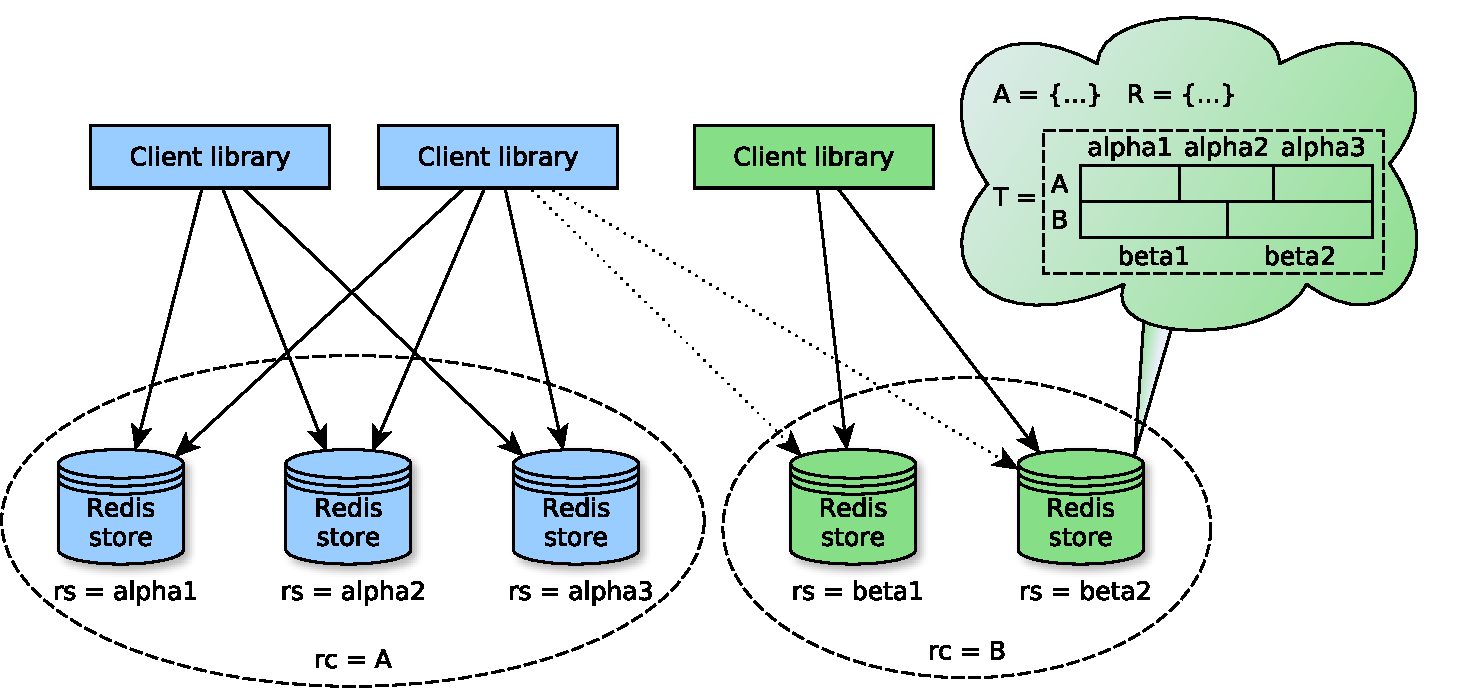
\includegraphics[width=1\textwidth]{architecture}
    \caption{Client library architecture}
    \label{fig:architecture}
  \end{minipage}
\end{figure}

\begin{figure}[t]
  \begin{minipage}{1\linewidth}
    \begin{lstlisting}[language=XML]
    <topology>
      <cluster id="A">
        <store id="alpha1" ip="127.0.0.1" port="6379"/>
        <store id="alpha2" ip="127.0.0.1" port="6382"/>
        <store id="alpha3" ip="127.0.0.1" port="6383"/>
      </cluster>

      <cluster id="B">
        <store id="beta1" ip="127.0.0.1" port="6380"/>
        <store id="beta2" ip="127.0.0.1" port="6384"/>
      </cluster>
    </topology>
    \end{lstlisting}
    \caption{Topology example in XML}
    \label{fig:topology}
  \end{minipage}
\end{figure}

\section{Database Schema}
\label{sec:database_schema}

Listing~\ref{lst:redis_database_schema_for_sor-set} contains the Redis schema
for storing the data on each shard. Underlined words represent hard-coded
strings, whereas non-underlined ones are to be replaced with their corresponding
value.

\begin{algorithm}[t]
\setcounter{algorithm}{0}
\small{
	\floatname{algorithm}{Listing}
	\caption{Redis database schema for SOR-Set}
 	\label{lst:redis_database_schema_for_sor-set}                       

 	\begin{algorithmic}[1]
 	  \State \underline{topology} $\rightarrow$ {$rc$:$rs$:$ip$:$port$} \Comment{Set}
 	  \State \underline{timestamp}:$rc$:$rs$ $\rightarrow$ $t$ \Comment{Integer string}
 	  \State \underline{element}:$rc.rs.id$ $\begin{aligned}[t]
                                              & \rightarrow \text{\underline{value}} \rightarrow e \\
                                              & \rightarrow \text{\underline{add.t}} \rightarrow t \\
                                              & \rightarrow \text{\underline{add.rc}} \rightarrow rc \\
                                              & \rightarrow \text{\underline{add.rs}} \rightarrow rs \\
                                              & \rightarrow \text{\underline{rmv.t}} \rightarrow t' \\
                                              & \rightarrow \text{\underline{rmv.rc}} \rightarrow rc' \\
                                              & \rightarrow \text{\underline{rmv.rs}} \rightarrow rs'
                                            \end{aligned}$ \Comment{Hash}
 	  \State \underline{index}:$rc$:$rs$ $\rightarrow$ [$t$:$rc.rs.id$] \Comment{List}
 	  \State \underline{ids}:$e$ $\rightarrow$ {$rc.rs.id$} \Comment{Set}
 	  \State \underline{element:next.id} $\rightarrow$ $id$ \Comment{Integer string}
	\end{algorithmic}
 }
\end{algorithm}

The topology is stored at key \underline{topology} as a set of strings, each
string representing a Redis store identified by the unique pair of cluster and
shard identifiers $rc$:$rs$ and $ip$:$port$ giving the machine address and port
number the Redis server is listening on. Each cell of the timestamp matrix,
$T[rc][rs]$, is stored at key \underline{timestamp}:$rc$:$rs$.

Instead of using different sets for added and removed tuples, they can be
combined and stored together as \textit{elements}. An element is created when a
new value is added to the set and has the following fields: the string value
$e$, the timestamp $t$, and the ids for the source replica cluster and shard
where the value was added, $(rc, rs)$. There are also equivalent fields for
retaining information about removal: timestamp $t'$ and shard $(rc', rs')$,
which are empty in the beginning. These last fields will be populated when
removing all $e$ elements from the set. Thus, an if an element has empty
\underline{rmv.t}, \underline{rmv.rc}, and \underline{rmv.rs} fields, then it
represents an $ADD$ tuple, otherwise it represents an $RMV$ one. Each element is
stored in the hash at key \underline{element}:$rc.rs.id$, where $rc.rs.id$
represents a global unique ID: $rc$ and $rs$ are the ids which uniquely
identifies the source shard and $id$ is a per-shard counter stored at
\underline{element:next.id} key which is incremented with each new element
insertion.

In Specification~\ref{alg:sor_set} of the SOR-Set, the \textit{merge} method
filters all tuples added or removed after a given timestamp. For this purpose,
an index is kept as a list of element ids sorted by their timestamp. With each
add or remove of an element at shard $(rc, rs)$, its id is appended to the list
\underline{index}:$rc$:$rs$. Since the index is kept per shard and timestamps at
each shard are monotonically increasing (adding and removing always increases
the local timestamp), \underline{index}:$rc$:$rs$ is guaranteed to be always
sorted. Thus, filtering new elements will be very efficient.

Adding the same value $e$ multiple times to the set creates a new element for
each operation. A second index stored at \underline{ids}:$e$ keeps all the
element ids corresponding to value $e$. As shown in the next section, this is
needed for $\textit{remove}(e)$ and $\textit{lookup}(e)$ methods.

\section{Operations Implementation}
\label{sec:operations}

The client is implemented in Java and communication with Redis is done through
the Jedis~\cite{jedis} library\footnote{The client library is property of 1\&1
Internet AG. Access to the source code can be allowed by request to 1\&1
Internet AG, M{\"u}nchen.}. This section presents the pseudocode for main
methods in the client's interface.

\subsection{Add}
\label{sec:ops_add}

Listing~\ref{alg:add} performs the \textit{add} operation.
First, the logical clock of the shard and the local id counter are incremented.
\texttt{incr} is an internal Redis command which increments the number stored at
the specified key by one\footnote{The rest of Redis commands will not be
described as their usage will be easily deduced from the context.}. Next, a
hash is created to store the new element and its expiration time is set. Last
two lines update the two indices previously discussed. An observation should be
made regarding \underline{index}:$rc$:$rs$: the elements are always pushed to
the left (the head) of the list, thus keeping it sorted in descending order by
the timestamp $t$. Section~\ref{sec:ops_merge} gives an explanation for this.
Procedure {\small\textsc{Add}} should execute atomically and in isolation with
other Redis commands on the store.

\subsection{Remove}
\label{sec:ops_remove}

Listing~\ref{alg:remove} contains the pseudocode for \textit{remove} method.
Again, removing an element $e$ from an SOR-Set consists in getting all $ADD(e)$
tuples and tagging them as removed. Thus, on line~3 all element ids for value
$e$ are retrieved using index \underline{ids}:$e$. Next, for each element stored
at \underline{element}:$gid$, if it is not yet expired (the key still exists in
the database), the corresponding fields are populated. Finally, the procedure
updates the expiration period of the element and pushes the new timestamp
together with the id to the index list. After removal, the new timestamp $t'$
will be ahead of the old one, $t$, in this list, which the expected behavior:
the remove happened after the add. Procedure {\small\textsc{Remove}} should
execute atomically and in isolation with other Redis commands on the store.

\begin{figure*}[t]
  \centering
  \noindent
  \begin{minipage}[t]{0.49\linewidth}
    \begin{algorithm}[H]
    \small{
    \floatname{algorithm}{Listing}
    \caption{Redis SOR-Set: \textit{add}}
    \label{alg:add}
    \centering
    \begin{algorithmic}[1]
 	  \Procedure{Add}{$e$, $rc$, $rs$, $ttl$}
 	    \State $t$ $\gets$ \texttt{incr} \underline{timestamp}:$rc$:$rs$
 	    \State $id$ $\gets$ \texttt{incr} \underline{element:next.id}
 	    \State \texttt{hmset} \underline{element}:$rc.rs.id$ $\begin{aligned}[t]
                                                               & \text{\underline{value} } e \\
                                                               & \text{\underline{add.t} } t \\
                                                               & \text{\underline{add.rc} } rc \\
                                                               & \text{\underline{add.rs} } rs
                                                              \end{aligned}$
        \State \texttt{expire} \underline{element}:$rc.rs.id$ $ttl$
        \State \texttt{lpush} \underline{index}:$rc$:$rs$ $t$:$rc.rs.id$
        \State \texttt{sadd} \underline{ids}:$e$ $rc.rs.id$
 	  \EndProcedure
	\end{algorithmic}
    }
    \end{algorithm}
  \end{minipage}
%   \qquad
  \noindent
  \begin{minipage}[t]{0.49\linewidth}
    \begin{algorithm}[H]
    \small{
    \floatname{algorithm}{Listing}
    \caption{Redis SOR-Set: \textit{remove}}
    \label{alg:remove}
    \centering
    \begin{algorithmic}[1]
 	  \Procedure{Remove}{$e$, $rc'$, $rs'$, $ttl$}
 	    \State $t'$ $\gets$ \texttt{incr} \underline{timestamp}:$rc'$:$rs'$
 	    \State $ids$ $\gets$ \texttt{smembers} \underline{ids}:$e$
 	    \ForAll{$gid$ \In $ids$}
 	      \If{\texttt{exists} \underline{element}:$gid$}
 	        \State \texttt{hmset} \underline{element}:$gid$ $\begin{aligned}[t]
                                                              & \text{\underline{rmv.t} } t' \\
                                                              & \text{\underline{rmv.rc} } rc' \\
                                                              & \text{\underline{rmv.rs} } rs'
                                                              \end{aligned}$
            \State \texttt{expire} \underline{element}:$gid$ $ttl$
            \State \texttt{lpush} \underline{index}:$rc'$:$rs'$ $t'$:$gid$
 	      \EndIf
 	    \EndFor
 	  \EndProcedure
	\end{algorithmic}
    }
    \end{algorithm}
  \end{minipage}
\end{figure*}

\subsection{Lookup}
\label{sec:ops_lookup}

Referring back to Specification~\ref{alg:sor_set}, the \textit{lookup} method
searches for the existence of at least one $ADD(e)$ tuple for which there is no
corresponding $RMV(e)$. If there is such tuple, then element $e$ is in the set.
This is exactly what Listing~\ref{alg:lookup} does. First, ids for all elements
$e$ are retrieved. Next, for each element $(e, t_1, rc_1, rs_1, t_1', rc_1',
rs_1')$, if it is an $ADD(e)$ tuple ($t_{1}' = \Null$, its removed timestamp is
not set) and does not exist any corresponding $RMV(e)$ tuple $(e, t_2, rc_2,
rs_2, t_2', rc_2', rs_2')$, such that $(t_1, rc_1, rs_1) = (t_2, rc_2, rs_2)$
and $t_2' \neq \Null$, then $\True$ is returned. Procedure
{\small\textsc{Lookup}} should execute atomically and in isolation with other
Redis commands on the store.

\begin{algorithm}[t]
\small{
	\floatname{algorithm}{Listing}
	\caption{Redis SOR-Set: \textit{lookup}}
 	\label{alg:lookup}

 	\begin{algorithmic}[1]
 	  \Function{Lookup}{$e$}
 	    \State $ids$ $\gets$ \texttt{smembers} \underline{ids}:$e$
 	    \ForAll{$gid_{1}$ \In $ids$}
 	      \If{\texttt{exists} \underline{element}:$gid_{1}$}
 	        \State ($t_{1}$, $rc_{1}$, $rs_{1}$, $t_{1}'$) $\gets$ \texttt{hmget} \underline{element}:$gid_{1}$ \underline{add.t} \underline{add.rc} \underline{add.rs} \underline{rmv.t}
 	        \If{$t_{1}' = \Null$}
 	          \State $lookup \gets \True$
 	          \ForAll{$gid_{2}$ \In $ids$}
 	            \If{\texttt{exists} \underline{element}:$gid_{2}$}
 	              \State ($\_$, $t_{2}$, $rc_{2}$, $rs_{2}$, $t_{2}'$, $rc_{2}'$, $rs_{2}'$) $\gets$ \texttt{hgetall} \underline{element}:$gid_{2}$
 	              \If{($t_{1}$, $rc_{1}$, $rs_{1}$) = ($t_{2}$, $rc_{2}$, $rs_{2}$) \Land $t_{2}' \neq \Null$}
 	                \State $lookup \gets \False$
 	                \State \Break
 	              \EndIf
 	            \EndIf
 	          \EndFor
 	          \If{$lookup = \True$}
 	            \State \Return \True
 	          \EndIf
 	        \EndIf
 	      \EndIf
 	    \EndFor
 	    \State \Return \False
 	  \EndFunction
	\end{algorithmic}
 }
\end{algorithm}

\subsection{Merge}
\label{sec:ops_merge}

The code for last method is given in Listing~\ref{alg:merge}. Here, lines 2 and
3 compute the version matrices for both the local and the remote clusters.
{\small\textsc{Version}} function previously introduced in
Specification~\ref{alg:sor_set} computes matrix $\tilde{T}$ cell by cell, by
fetching \underline{timestamp}:$rc_{i}$:$rc_{i}^{j}$, $\forall rc_{i}, \forall
rs_{i}^{j}, j \in \{1,\ldots,|rc_{i}|\}$ from each store in the cluster and by
selecting the minimum one (or maximum for row $rc_{i}^{j} = rc$).

\begin{algorithm}[b!]
\small{
	\floatname{algorithm}{Listing}
	\caption{Redis SOR-Set: \textit{merge} (part 1)}
 	\label{alg:merge}

 	\begin{algorithmic}[1]
 	  \Procedure{Merge}{$rc_{x}$, $rc_{y}$}
 	    \State $\tilde{T}_{x}$ $\gets$ \Call{Version}{$rc_{x}$}
 	    \State $\tilde{T}_{y}$ $\gets$ \Call{Version}{$rc_{y}$}
 	    \State $updates$ $\gets$ \Call{GetUpdates}{$rc_{y}$, $\tilde{T}_{x}$}
 	    \State \Call{AddUpdates}{$rc_{x}$, $hash_{x}$, $updates$}
 	    \State \Call{UpdateTimestamps}{$rc_{x}$, $\tilde{T}_{y}$}
 	  \EndProcedure

      \Function{Version}{$rc$}
        \ForAll{$rc_{i}$ \In clusters()}
          \ForAll{$rs_{i}^{j}$ \In shards($rc_{i}$)}
            \If{$rc_{i} = rc$}
              \State $\tilde{T}[rc_{i}][rs_{i}^{j}] \gets -\infty$
            \Else
              \State $\tilde{T}[rc_{i}][rs_{i}^{j}] \gets +\infty$
            \EndIf
 	        \ForAll{$store$ \In shards($rc$)}
 	          \State $t$ $\gets$ $store$.\texttt{get} \underline{timestamp}:$rc_{i}$:$rc_{i}^{j}$
 	          \If{$rc_{i} = rc$}
                \State $\tilde{T}[rc_{i}][rs_{i}^{j}] \gets max(\tilde{T}[rc_{i}][rs_{i}^{j}], t)$
              \Else
                \State $\tilde{T}[rc_{i}][rs_{i}^{j}] \gets min(\tilde{T}[rc_{i}][rs_{i}^{j}], t)$
              \EndIf
 	        \EndFor
 	      \EndFor
 	    \EndFor
 	    \State \Return $\tilde{T}$
 	  \EndFunction

      \Function{GetUpdates}{$rc$, $\tilde{T}$}
 	    \ForAll{$store$ \In shards($rc$)}
 	      \ForAll{$rc_{i}$ \In clusters()}
 	        \ForAll{$rs_{i}^{j}$ \In shards($rc_{i}$)}
 	          \State $list \gets store.\texttt{llen}$ \underline{index}:$rc_{i}$:$rs_{i}^{j}$
 	          \State $page \gets min(PAGE, list)$
 	          \For{($start \gets -list$; $start < 0$; $start \gets start + page$)}
 	            \State $tgids$ $\gets$ $store$.\texttt{lrange} \underline{index}:$rc_{i}$:$rs_{i}^{j}$ $start$ $(start + page - 1)$
 	            \State $k$ $\gets$ $bsearch(tgids, \tilde{T}[rc_{i}][rs_{i}^{j}])$
                \For{($u \gets 0$, $t$:$gid$ $\gets$ $tgids[u]$; $u < k$; $u \gets u + 1$)}
 	              \State ($e$, $t$, $rc$, $rs$, $t'$, $rc'$, $rs'$)$_{u} \gets$ $store$.\texttt{hgetall} \underline{element}:$gid$
 	              \State $ttl$ $\gets$ $store$.\texttt{ttl} \underline{element}:$gid$
 	              \State $updates \gets updates$ + (($e$, $t$, $rc$, $rs$, $t'$, $rc'$, $rs'$)$_{u}$, $gid$, $ttl$)
                \EndFor
                \If{$k < page$}
                  \State \Break
                \EndIf
 	          \EndFor
 	        \EndFor
 	      \EndFor
 	    \EndFor
 	    \State \Return updates
 	  \EndFunction
 	  \algstore{alg:merge:break}
    \end{algorithmic}
 }
\end{algorithm}

\begin{algorithm}[t]
\small{
	\floatname{algorithm}{Listing}
	\caption{Redis SOR-Set: \textit{merge} (part 2)}

 	\begin{algorithmic}[1]
      \algrestore{alg:merge:break}

      \Procedure{AddUpdates}{$rc$, $hash$, $updates$}
        \ForAll{(($e$, $t$, $rc$, $rs$, $t'$, $rc'$, $rs'$)$_{u}$, $gid$, $ttl$) \In $updates$}
 	      \State $j$ $\gets$ $hash(e)$
 	      \State $store$ $\gets$ $shards(rc)[j]$
 	      \State $store$.\texttt{hmset} \underline{element}:$gid$ ($e$, $t$, $rc$, $rs$, $t'$, $rc'$, $rs'$)$_{u}$
 	      \State $store$.\texttt{expire} \underline{element}:$gid$ $ttl$
 	      \If{$t' = \Null$}
 	        \State $store$.\texttt{lpush} \underline{index}:$rc$:$rs$ $t$:$gid$
 	      \Else
 	        \State $store$.\texttt{lpush} \underline{index}:$rc'$:$rs'$ $t'$:$gid$
 	      \EndIf
 	      \State $store$.\texttt{sadd} \underline{ids}:$e$ $gid$
 	    \EndFor
 	  \EndProcedure

      \Procedure{UpdateTimestamps}{$rc$, $\tilde{T}$}
        \ForAll{$store$ \In shards($rc$)}
          \ForAll{$rc_{i}$ \In clusters()}
            \ForAll{$rs_{i}^{j}$ \In shards($rc_{i}$)}
              \State $t$ $\gets$ $store$.\texttt{get} \underline{timestamp}:$rc_{i}$:$rs_{i}^{j}$
              \State $store$.\texttt{set} \underline{timestamp}:$rc_{i}$:$rs_{i}^{j}$ max($t$, $\tilde{T}[rc_{i}][rs_{i}^{j}]$)
            \EndFor
          \EndFor
        \EndFor
      \EndProcedure
	\end{algorithmic}
 }
\end{algorithm}

Based on the local version matrix $\tilde{T}_{x}$, next the procedure fetches
the updates from remote cluster $rc_{y}$ using {\small\textsc{GetUpdates}}
function. Remember that each store keeps an index of element ids ($ADD$ and
$RMV$ tuples), sorted in descending order by their timestamp, i.e. the newer
elements are at the beginning of the list. Since the goal is to filter all
elements newer than a given $t = \tilde{T}_{x}[rc_{i}][rs_{i}^{j}]$ value, 
\textit{pages} (or segments) are fetched starting from the head of this list
until the first value greater than $t$ is found. All elements before this value
in the list are the relevant updates. Inside each page, searching for $t$ can be
done using a binary search function because the list is already sorted. The
reason why it is sorted in descending order is because Redis store should not
block until fetching all pages. The store can process other requests meanwhile
and, if newer element ids are added to the index, this will shift the offsets
for the subsequent pages. Alternatively, the list could have been kept sorted in
ascending order and fetching pages would have been done starting from the end of
it. However, the complexity of one page request would be in this case
proportional to the start offset of the page as stated in the Redis
documentation for \texttt{lrange} command~\cite{redis}.

Thus, considering that $p$ pages are fetched in total until $t$ is found and
that the page size is $page$, the complexity of {\small\textsc{GetUpdates}}
function is $\mathcal{O}(p \times page)$. Another option would have been to use
a Redis sorted set instead of a list. In this case, the complexity for each
update to the index is $\mathcal{O}(log(n))$, instead of $\mathcal{O}(1)$, where
$n$ is the index size, while getting all $m$ ids newer than $t$ is an
$\mathcal{O}(log(n)+m)$ operation. Since the page size $page$ is a heuristic
that can be determined if we know the approximate number of updates between
merge operations, it can be argued that just a few number of pages are needed to
be fetched, and thus $\mathcal{O}(p \times page) \approx \mathcal{O}(page) <
\mathcal{O}(log(n)+m)$.

Continuing with the \textit{merge} method, $updates$ contains all elements from
the remote cluster, $rc_{y}$, which are missing from the local one, $rc_{x}$.
In this list, elements coming from any $rs_{y}^{j}$ store are found in the same
relative order in which they were in the index of that store. Also, in
conformance to the garbage collection mechanism described in
Section~\ref{sec:garbage_collection}, the procedure fetches the TTLs together
with the elements\footnote{Redis command \texttt{ttl} retrieves the remaining
time-to-live for the given key.}. The next subroutine,
{\small\textsc{AddUpdates}}, distributes these elements from $updates$ to the
stores in the local cluster according to $hash_{x}$ function. Adding an update
element to the store is an operation similar to \textit{add}, except that the
logical clock is not incremented and the TTLs are the ones retrieved before.
Setting the logical clocks is done at the end in the
{\small\textsc{UpdateTimestamps}} subroutine according to the formula $T_{x}^{j}
\coloneqq max(T_{x}^{j}, \tilde{T}_{y}), \forall j \in \{1,\ldots,|rc_{x}|\}$.

Procedure {\small\textsc{AddUpdates}} and updating the timestamps in lines
52--53 should execute atomically and in isolation with other Redis commands on
that store.

\section{Unit Tests}
\label{sec:unit_tests}

\begin{figure}[t!]
  \noindent
  \centering
  \subcaptionbox{$ADD \rightarrow RMV$}{
	\begin{minipage}[t][0.05\textwidth]{0.35\textwidth}
	   \centering
	   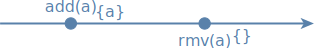
\includegraphics[width=1\textwidth]{test-basic-02}
	\end{minipage}}
  \qquad
  \subcaptionbox{$RMV \rightarrow ADD$}{
	\begin{minipage}[t][0.05\textwidth]{0.35\textwidth}
	   \centering
	   \includegraphics[width=1\textwidth]{test-basic-04}
	\end{minipage}}
  \\ \vspace*{1em}
  \subcaptionbox{$ADD$ $\leadsto$ directly}{
	\begin{minipage}[t][0.1\textwidth]{0.35\textwidth}
	   \centering
	   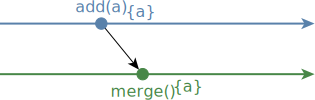
\includegraphics[width=1\textwidth]{test-basic-05}
	\end{minipage}}
  \qquad
  \subcaptionbox{$ADD$ $\leadsto$ indirectly}{
	\begin{minipage}[t][0.1\textwidth]{0.35\textwidth}
	   \centering
	   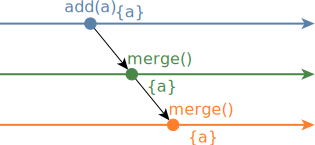
\includegraphics[width=1\textwidth]{test-basic-06}
	\end{minipage}}
  \\ \vspace*{1em}
  \subcaptionbox{$RMV$ $\leadsto$ directly}{
	\begin{minipage}[t][0.1\textwidth]{0.35\textwidth}
	   \centering
	   \includegraphics[width=1\textwidth]{test-basic-07}
	\end{minipage}}
  \qquad
  \subcaptionbox{$RMV$ $\leadsto$ indirectly}{
	\begin{minipage}[t][0.1\textwidth]{0.35\textwidth}
	   \centering
	   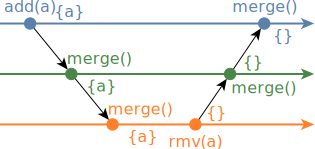
\includegraphics[width=1\textwidth]{test-basic-08}
	\end{minipage}}
  \\ \vspace*{1em}
  \subcaptionbox{$ADD \parallel RMV$ directly}{
	\begin{minipage}[t][0.1\textwidth]{0.35\textwidth}
	   \centering
	   \includegraphics[width=1\textwidth]{test-basic-09}
	\end{minipage}}
  \qquad
  \subcaptionbox{$ADD \parallel RMV$ indirectly}{
	\begin{minipage}[t][0.1\textwidth]{0.35\textwidth}
	   \centering
	   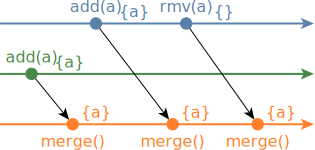
\includegraphics[width=1\textwidth]{test-basic-10}
	\end{minipage}}
\caption{Basic correctness tests for SOR-Set}
\label{fig:basic_tests}
\end{figure}

To prove the correctness of the SOR-Set, three categories of tests were devised:
i) basic set operations, ii) garbage collection, and iii) fault tolerance. For each
replica both single-shard and multi-shards clusters were used.

The purpose of the first set, depicted in Figure~\ref{fig:basic_tests}, was
to test the results of update operations in different scenarios. After each
update, assertions compared the boolean value returned by the
$\textit{lookup}(a)$ method with the expected one. The states of the replicas at
each step are depicted in curly braces.

The following tests, in Figure~\ref{fig:gc_tests}, show that the garbage
collection mechanism conforms with the tuple expiration theorem. Here, the
dashed lines denote the lifetime of each tuple.

\begin{figure}[t]
  \noindent
  \centering
  \subcaptionbox{$ADD \rightarrow RMV$ expire locally}{
	\begin{minipage}[t][0.1\textwidth]{0.35\textwidth}
	   \centering
	   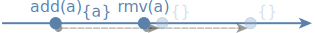
\includegraphics[width=1\textwidth]{test-gc-01}
	\end{minipage}}
  \qquad
  \subcaptionbox{$RMV \rightarrow ADD$ expire locally}{
	\begin{minipage}[t][0.1\textwidth]{0.35\textwidth}
	   \centering
	   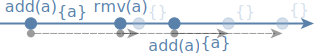
\includegraphics[width=1\textwidth]{test-gc-02}
	\end{minipage}}
  \\ \vspace*{1.5em}
  \subcaptionbox{$ADD \rightarrow RMV$ expire remotely}{
	\begin{minipage}[t][0.1\textwidth]{0.35\textwidth}
	   \centering
	   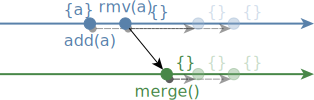
\includegraphics[width=1\textwidth]{test-gc-03}
	\end{minipage}}
  \qquad
  \subcaptionbox{$RMV \rightarrow ADD$ expire remotely}{
	\begin{minipage}[t][0.1\textwidth]{0.35\textwidth}
	   \centering
	   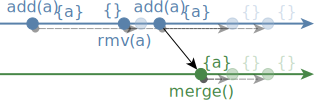
\includegraphics[width=1\textwidth]{test-gc-04}
	\end{minipage}}
\caption{Garbage collection tests for SOR-Set}
\label{fig:gc_tests}
\end{figure}

The last group of tests in Figure~\ref{fig:fail_tests} proves the resilience
of the SOR-Set in the presence of failures. The first two tests show that
propagation of updates stops at the failed stores, while the next two show that
missed updates are recovered during subsequent \textit{merge} operations.
Synchronization between replicas containing either failed stores in the remote
cluster from where the updates are pulled or in the local cluster is also
not affected, as shown in the last two tests.

\begin{figure}[t]
  \noindent
  \centering
  \subcaptionbox{$ADD$ $\not\leadsto$ at the failed store}{
	\begin{minipage}[t][0.1\textwidth]{0.35\textwidth}
	   \centering
	   \includegraphics[width=1\textwidth]{test-fail-01}
	\end{minipage}}
  \qquad
  \subcaptionbox{$RMV$ $\not\leadsto$ at the failed store}{
	\begin{minipage}[t][0.1\textwidth]{0.35\textwidth}
	   \centering
	   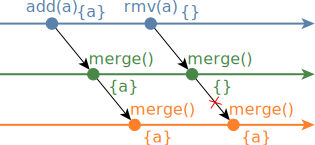
\includegraphics[width=1\textwidth]{test-fail-02}
	\end{minipage}}
  \\ \vspace*{1.5em}
  \subcaptionbox{$ADD$ $\leadsto$ after source fails}{
	\begin{minipage}[t][0.1\textwidth]{0.35\textwidth}
	   \centering
	   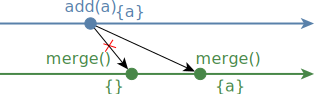
\includegraphics[width=1\textwidth]{test-fail-03}
	\end{minipage}}
  \qquad
  \subcaptionbox{$RMV$ $\leadsto$ after source fails}{
	\begin{minipage}[t][0.1\textwidth]{0.35\textwidth}
	   \centering
	   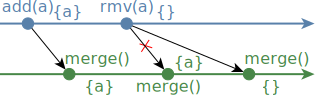
\includegraphics[width=1\textwidth]{test-fail-04}
	\end{minipage}}
  \\ \vspace*{1.5em}
  \subcaptionbox{Store failures in remote cluster}{
	\begin{minipage}[t][0.1\textwidth]{0.35\textwidth}
	   \centering
	   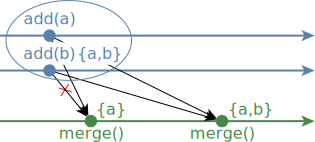
\includegraphics[width=1\textwidth]{test-fail-05}
	\end{minipage}}
  \qquad
  \subcaptionbox{Store failures in local cluster}{
	\begin{minipage}[t][0.1\textwidth]{0.35\textwidth}
	   \centering
	   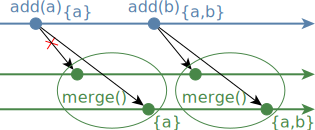
\includegraphics[width=1\textwidth]{test-fail-06}
	\end{minipage}}
\caption{Fault tolerance tests for SOR-Set}
\label{fig:fail_tests}
\end{figure}

\section{Evaluation}
\label{sec:evaluation}

This section presents the results obtained for evaluating the SOR-Set client
library. The test systems were equipped with Intel Xeon E5520 dual quad core
CPUs with HyperThreading support running at 2.27GHz and with 24GB of RAM,
interconnected through 1Gbps network interfaces. For the datastore, Redis
version 2.6.0-rc6 was used.

The purpose of the first benchmark was to measure how the average time needed to
merge two replicated sets changes as the database size increases. Test
configuration included 16 Redis instances running on one machine representing
Replica~A, each instance storing one shard of the set. For Replica~B another
machine with identical configuration was used. The client library was deployed
on a third machine. The methodology for measuring was: add 1 million 32-byte
uniform randomly generated elements to Replica~A, measure the time for merging
into Replica~B using a pool of 16 threads, and then repeat the process.

\begin{figure}[t]
  \centering
  \begin{minipage}{1\linewidth}
    \centering
    \includegraphics[width=0.9\textwidth]{bench_delta}
    \caption{Delta-based synchronization}
    \label{fig:bench_delta}
  \end{minipage}
\end{figure}

\begin{figure}[t!]
  \centering
  \begin{minipage}{1\linewidth}
    \centering
    \includegraphics[width=0.9\textwidth]{bench_ops}
    \caption{Throughput for set operations}
    \label{fig:bench_ops}
  \end{minipage}
\end{figure}

Results are presented in Figure~\ref{fig:bench_delta}. Here were also
included the average timings for each subroutine  of the \textit{merge}
procedure described in Listing~\ref{alg:merge} relevant to these measurements:
getting the pages with element ids, fetching the actual elements from the remote
cluster, and adding the elements to the local cluster. The first observation is
that delta-based synchronization algorithm scales well with the database size.
Since the number of updates between each merge operation was constant, the
timings were also relatively constant. Thus, the \textit{merge} procedure has a
time complexity proportional to the number of updates, i.e. delta size, and not
to the database size. Second, from this graphic plot the average throughput for
merging can be computed to 125,000 update elements per second.

The second benchmark measured the average throughput of all the basic set
operations. For this, a machine with 16 Redis servers acting as a replica
cluster was used. The client library was deployed on another machine to perform
the test: add 1 million 32-byte uniform randomly generated elements to the set,
look them up, remove them, and then repeat the process with more elements.
The drop in throughput in Figure~\ref{fig:bench_ops} can have one of two causes:
either the operations have time complexity proportional to the database size, or
Redis incurs performance penalty as its database increases.
Specifications~\ref{alg:add}, \ref{alg:remove}, and \ref{alg:lookup} show that
only $\mathcal{O}(1)$ Redis operations are used, assuming that same values are
not inserted in the set. This a reasonable assumption since 10 million elements
are generated, each chosen with the same probability from a $2^{8 \times 32}$
space, and thus leading to a low chance of collision. Therefore, updating the
indices is on average a constant operation: \underline{ids}:$e$ contains only
one id and \texttt{lpush} \underline{index}:$rc$:$rs$ is constant. The decline
in performance may be attributed to Redis' management of its internal
structures, such as the global hash table which stores all the keys. As the
database size increases, Redis has to adjust the capacity of this hash, making a
simple \texttt{get} operation on any key costly.

The reason why a better throughput was obtained for \textit{merge} has two
causes. First, each of \textit{add}, \textit{lookup}, and \textit{remove} is
implemented using Lua scripts\footnote{Redis supports Lua scripts starting from
version 2.6.0.} for which Redis guarantees to execute in an atomic way. As
discussed in Section~\ref{sec:operations}, this was needed to ensure that
updating the elements and the indices in the database does not interleave with
other Redis commands. 

Second, fetching the elements and distributing the updates
in the \textit{merge} procedure are done using pipelines: sending multiple Redis
commands without waiting for a reply from the server, thus saving the
round-trip-time of each request. Unfortunately, the same technique cannot be
used for the other procedures because both \textit{add} and \textit{remove}
increment a counter to generate the id for each element, while \textit{lookup}
must first fetch all ids of one element. This means we have to wait for a reply
from Redis before calling the subsequent commands, i.e. basic set operations
contain synchronous calls to Redis which make them unsuitable for pipelining. 
This is not considered to be a problem since these procedures are independent
and are usually issued by different clients, as opposed to the subroutines of
one \textit{merge} call.